\documentclass[svgnames,11pt]{beamer}
\input{/home/tof/Documents/Cozy/latex-include/preambule_commun.tex}
\input{/home/tof/Documents/Cozy/latex-include/preambule_beamer.tex}
%\usepackage{pgfpages} \setbeameroption{show notes on second screen=left}
\author[]{Christophe Viroulaud}
\title{Programmation dynamique\\suite de Fibonacci}
\date{\framebox{\textbf{Algo 24}}}
%\logo{}
\institute{Terminale - NSI}

\begin{document}
\begin{frame}
\titlepage
\end{frame}
\begin{frame}
    \frametitle{}
    $$
        F_n = \left\{
        \begin{array}{ll}
            F_0 = 0                 & \mbox{si } n=0 \\
            F_1=1                   & \mbox{si } n=1 \\
            F_{n} = F_{n-1}+F_{n-2} & \mbox{si } n>1 \\
        \end{array}
        \right.
    $$
    \begin{framed}
        \centering Comment obtenir un calcul efficace des termes de la suite?
    \end{framed}
\end{frame}

\section{Mise en évidence du problème}
\begin{frame}
    \frametitle{Mise en évidence du problème}
    $$
        F_n = \left\{
        \begin{array}{ll}
            F_0 = 0                 & \mbox{si } n=0 \\
            F_1=1                   & \mbox{si } n=1 \\
            F_{n} = F_{n-1}+F_{n-2} & \mbox{si } n>1 \\
        \end{array}
        \right.
    $$
\begin{activite}
Écrire la fonction \textbf{\texttt{fibo(n: int) $\rightarrow$ int}} qui calcule le terme de rang \textbf{\texttt{n}} de la suite.
\end{activite}
\end{frame}
\begin{frame}[fragile]
    \frametitle{Correction}

\begin{center}
\begin{lstlisting}[language=Python , basicstyle=\ttfamily\small, xleftmargin=2em, xrightmargin=2em]
def fibo(n: int)->int:
    """
    calcule le terme de rang n
    de la suite de Fibonacci
    """
    if n == 0:
        return 0
    elif n == 1:
        return 1
    else:
        return fibo(n-1) + fibo(n-2)
\end{lstlisting}
\end{center}

\end{frame}
\begin{frame}
    \frametitle{}
    \begin{center}
    \centering
    \includegraphics[width=10cm]{ressources/fibo1.png}
    \captionof{figure}{Pour \textbf{\texttt{n = 8}}}
    \label{IMG}
    \end{center}
\end{frame}

\begin{frame}
    \frametitle{}
    \begin{center}
        \centering
        \includegraphics[width=11cm]{ressources/nb-appels.png}
        \captionof{figure}{Nombre d'appels en fonction de n}
    \end{center}
\end{frame}
\begin{frame}
    \frametitle{}

    \begin{aretenir}[Remarque]
    La fonction calcule plusieurs fois la même valeur. Le nombre d'appels augmente de manière exponentielle.
    \end{aretenir}

\end{frame}
\section{Programmation dynamique}
\subsection{Principe}
\begin{frame}
    \frametitle{Programmation dynamique - Principe}
La programmation dynamique:
    \begin{itemize}
        \item s'appuie sur le principe de \textbf{diviser pour régner},
        \item stocke les résultats intermédiaires pour éviter de les calculer à nouveau.
    \end{itemize}

\end{frame}
\begin{frame}
    \frametitle{}

    \begin{aretenir}[Remarque]
    \textbf{Richard Bellman} développe cette stratégie algorithmique dès les années 1950.
    \end{aretenir}

    
\end{frame}
\begin{frame}
    \frametitle{}

    \begin{aretenir}[Remarque]
        En toute rigueur, on n'applique pas tout à fait le principe \textbf{diviser pour régner} dans la suite de Fibonacci: les problèmes ne sont pas indépendants.
        \end{aretenir}

\end{frame}
\subsection{Approche top-down}
\begin{frame}
    \frametitle{Approche top-down}

    
    \begin{aretenir}[]
    Dans l'approche \textbf{top-down (ou descendante)}, on:
    \begin{itemize}
        \item applique une méthode récursive,
        \item stocke les résultats des appels récursifs (\textbf{mémoïsation}).
    \end{itemize}
    \end{aretenir}

\end{frame}
\begin{frame}[fragile]
    \frametitle{}
\begin{center}
\begin{lstlisting}[language=Python , basicstyle=\ttfamily\small, xleftmargin=0.2em, xrightmargin=0em]
def fibo_td(n: int, track: list) -> int:
    # déjà calculé
    if track[n] > 0:
        return track[n]
    if n == 0:
        track[0] = 0
        return track[0]
    elif n == 1:
        track[1] = 1
        return track[1]
    else:
        track[n] = fibo_td(n-1, track) + \
                    fibo_td(n-2, track)
        return track[n]
\end{lstlisting}
\captionof{code}{\centering \textbf{\texttt{track}} stocke les résultats déjà calculés.}
\end{center}
\end{frame}
\begin{frame}[fragile]
    
\begin{center}
    \begin{lstlisting}[language=Python , basicstyle=\ttfamily\small, xleftmargin=0.2em, xrightmargin=2em]
n = 20
track = [-1 for _ in range(n+1)]
fibo_td(n, track)
\end{lstlisting}
\captionof{code}{Appel de la fonction}
    \label{CODE}
    \end{center}
\end{frame}


\begin{frame}
    \frametitle{}

    \begin{center}
        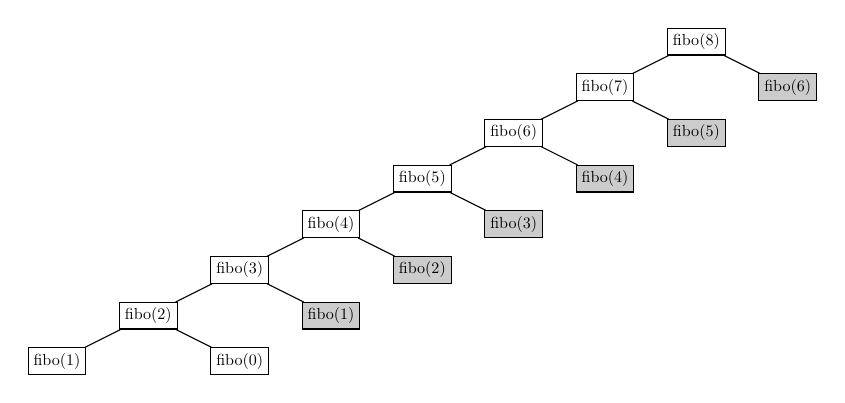
\begin{tikzpicture}[scale=0.58, transform shape]
            \node[draw] (A) at (0,0) {fibo(8)};
            \node[draw] (B) at (-2,-1) {fibo(7)};
            \node[draw,fill=gray!40] (C) at (2,-1) {fibo(6)};
            \node[draw] (D) at (-4,-2) {fibo(6)};
            \node[draw,fill=gray!40] (E) at (0,-2) {fibo(5)};
            \node[draw] (F) at (-6,-3) {fibo(5)};
            \node[draw,fill=gray!40] (H) at (-2,-3) {fibo(4)};
            \node[draw] (I) at (-8,-4) {fibo(4)};
            \node[draw,fill=gray!40] (J) at (-4,-4) {fibo(3)};
            \node[draw] (K) at (-10,-5) {fibo(3)};
            \node[draw,fill=gray!40] (M) at (-6,-5) {fibo(2)};
            \node[draw] (O) at (-12,-6) {fibo(2)};
            \node[draw,fill=gray!40] (P) at (-8,-6) {fibo(1)};
            \node[draw] (Q) at (-14,-7) {fibo(1)};
            \node[draw] (R) at (-10,-7) {fibo(0)};

            \draw (A) -- (B);
            \draw (A) -- (C);
            \draw (B) -- (D);
            \draw (B) -- (E);
            \draw (D) -- (F);
            \draw (D) -- (H);
            \draw (F) -- (I);
            \draw (F) -- (J);
            \draw (I) -- (K);
            \draw (I) -- (M);
            \draw (K) -- (O);
            \draw (K) -- (P);
            \draw (O) -- (Q);
            \draw (O) -- (R);
        \end{tikzpicture}
        \captionof{figure}{Appels récursifs pour $n=8$}
        \label{moncode}
    \end{center}

\end{frame}
\begin{frame}
    \frametitle{}

    \begin{center}
        \centering
        \includegraphics[width=10cm]{ressources/nb-appels-dyn.png}
        \captionof{figure}{Nombre d'appels en fonction de \textbf{\texttt{n}}}
    \end{center}

\end{frame}
\subsection{Approche bottom-up}
\begin{frame}
    \frametitle{Approche bottom-up}

    
    \begin{aretenir}[]
    Dans l'approche \textbf{bottom-up (ou ascendante)}, on:
    \begin{itemize}
        \item applique une méthode itérative,
        \item résout d'abord les petits problèmes.
    \end{itemize}
    \end{aretenir}

\end{frame}

\begin{frame}[fragile]
    \frametitle{}

\begin{center}
\begin{lstlisting}[language=Python , basicstyle=\ttfamily\small, xleftmargin=0.2em, xrightmargin=0em]
def fibo_bu(n: int) -> int:
    # résultats déjà calculés
    track = [0 for _ in range(n+1)]
    track[1] = 1

    # calcule de proche en proche
    for i in range(2, n+1):
        track[i] = track[i-1] + track[i-2]

    return track[n]
\end{lstlisting}
\captionof{code}{\textbf{\texttt{track}} stocke les résultats.}
\label{CODE}
\end{center}

\end{frame}
\begin{frame}
    \frametitle{}

    \begin{aretenir}[]
    La complexité en temps de cette approche est équivalente à celle précédente: on ne calcule chaque sous-problème qu'une seule fois.
    \end{aretenir}

\end{frame}
\subsection{Optimisation}
\begin{frame}
    \frametitle{Optimisation}
\begin{aretenir}[Remarque]
La complexité en espace dépend de la taille du tableau \textbf{\texttt{track}}. Cependant, si seul le résultat final nous intéresse, il est possible d'optimiser l'approche ascendante.
\end{aretenir}

\end{frame}

\begin{frame}[fragile]
    \frametitle{}
\begin{center}
\begin{lstlisting}[language=Python , basicstyle=\ttfamily\small, xleftmargin=0.2em, xrightmargin=0em]
def fibo_bu(n: int) -> int:
    track0 = 0
    track1 = 1

    for i in range(2, n+1):
        # calcule de proche en proche
        track0, track1 = track1, track0 + track1

    return track1
\end{lstlisting}
\captionof{code}{On ne garde en mémoire que les deux dernières valeurs.}
\label{CODE}
\end{center}
\end{frame}
\end{document}